\documentclass{beamer}
\usetheme{Madrid}
\usepackage[utf8]{inputenc}

\usepackage{algorithmic}
\usepackage{algorithm}
\renewcommand{\algorithmicrequire}{\textbf{Input:}}
\renewcommand{\algorithmicensure}{\textbf{Output:}}

\usepackage{amssymb}
\usepackage{amsfonts}
\usepackage{amsmath}
\newcommand{\argmin}{\mathop{\mathrm{arg\,min}}\limits}
\newcommand{\argmax}{\mathop{\mathrm{arg\,max}}\limits}
\newcommand{\mymin}{\mathop{\mathrm{min}}\limits}

\graphicspath{ {./images/} }

\usepackage{xspace}

\usepackage{multirow}
\usepackage{booktabs}

\newcommand{\anpcp}{$\alpha$N$p$CP\xspace}
\newcommand{\pcp}{$p$CP\xspace}
\newcommand{\pdp}{$p$DP\xspace}

\title[A heuristic for the \anpcp]{A heuristic for the $\alpha$-neighbor $p$-center problem}
\author{Eduardo Salazar, Roger Z. Ríos}
\institute[]{
    Department of Mechanical and Electrical Engineering \\
    Universidad Autónoma de Nuevo León \\
    San Nicolás de los Garza, N.L.
}
\date[X CSMIO]{
    X Congreso de la Sociedad Mexicana de Investigación de Operaciones \\ 
    October 19th, 2021
}

\begin{document}

\begin{frame}
    \titlepage
\end{frame}

\begin{frame}{Outline}
    \tableofcontents
\end{frame}

\section{Problem statement and motivation}

\begin{frame}{$\alpha$-Neighbor $p$-Center Problem (\anpcp)}
    \framesubtitle{Problem formulation}
    Generalization of the classical $p$-center problem (\pcp), in which the goal is to select $p$ centers such that the maximum distance of a non-center point to its $\alpha$-th nearest center is minimized.
    
    Note that setting $\alpha = 1$ corresponds to the \pcp.
\end{frame}

\begin{frame}{$\alpha$-Neighbor $p$-Center Problem (\anpcp)}
    \framesubtitle{Problem formulation}
    
    $n = 20$ \\
    $m = 10$ \\
    $p = 5$ \\
    $\alpha = 2$
    
    \begin{figure}
        \centering
        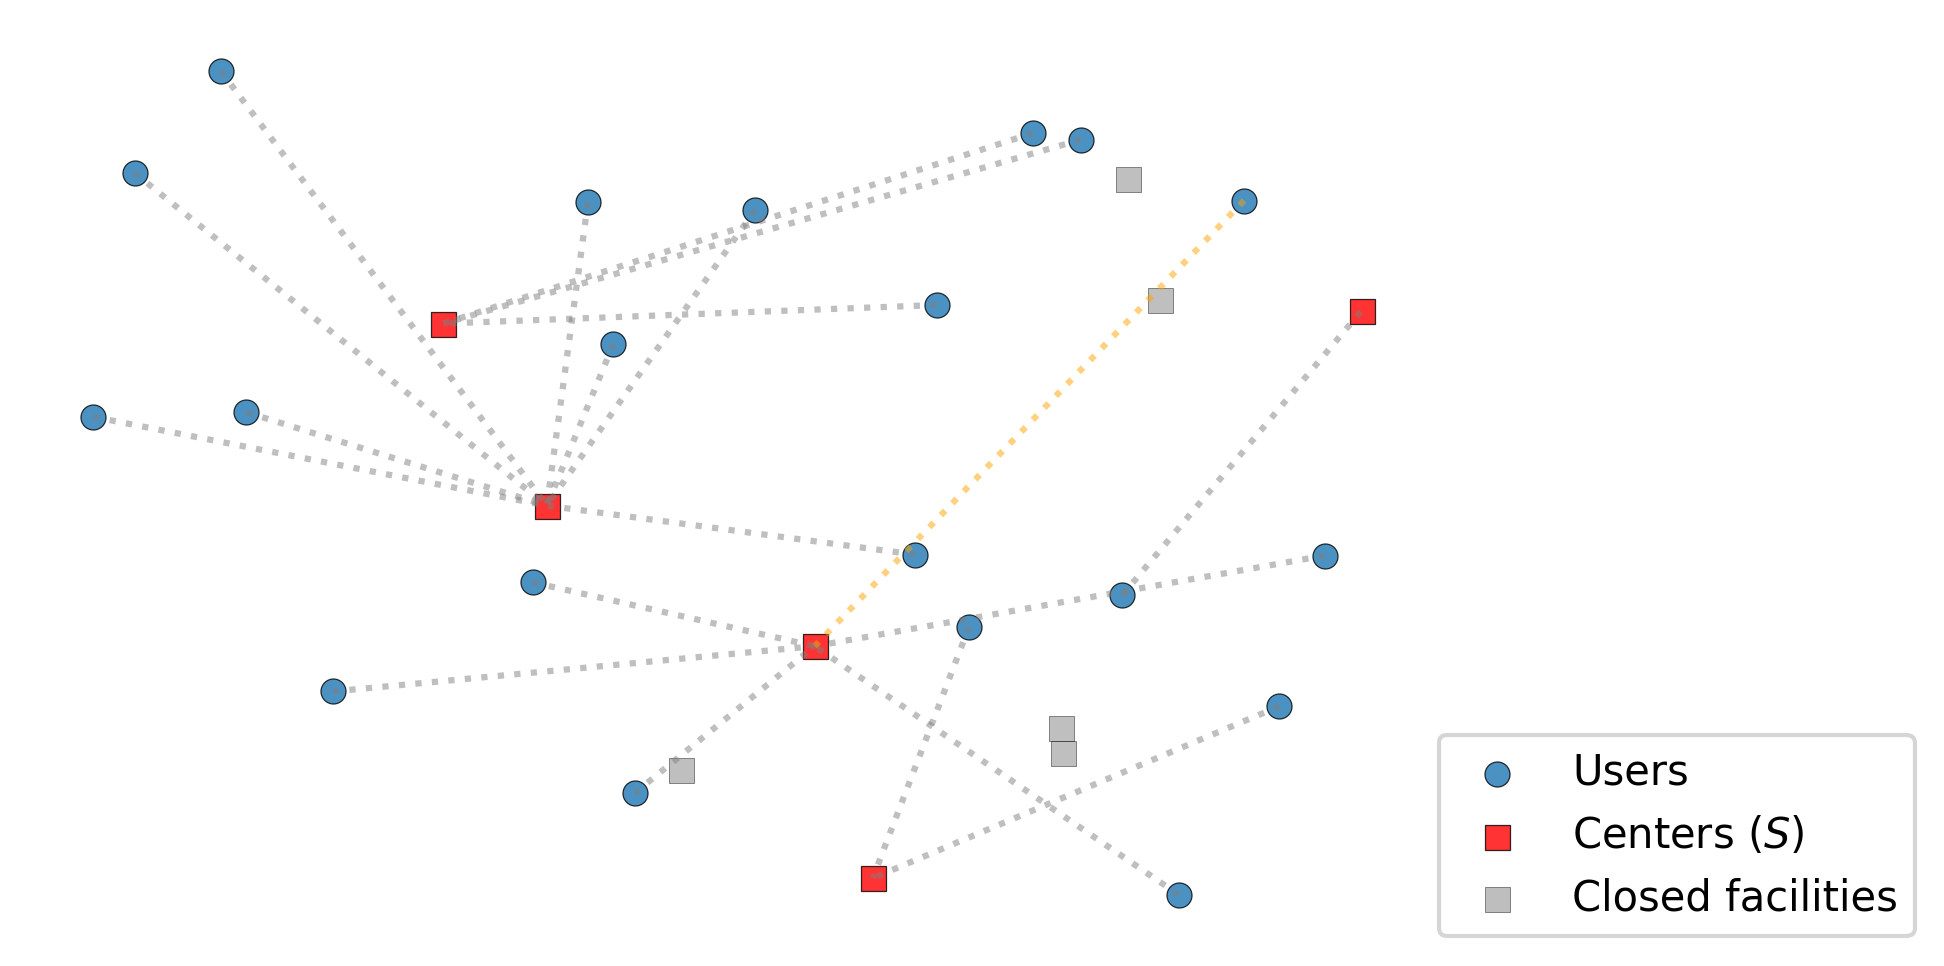
\includegraphics[scale=0.7]{2npcp}
        \label{fig:2npcp}
    \end{figure}
\end{frame}

\begin{frame}{$\alpha$-Neighbor $p$-Center Problem (\anpcp)}
    \framesubtitle{Problem formulation}
    
    $n = 20$ \\
    $m = 10$ \\
    $p = 5$ \\
    $\alpha = 1$ (PCP)
    
    \begin{figure}
        \centering
        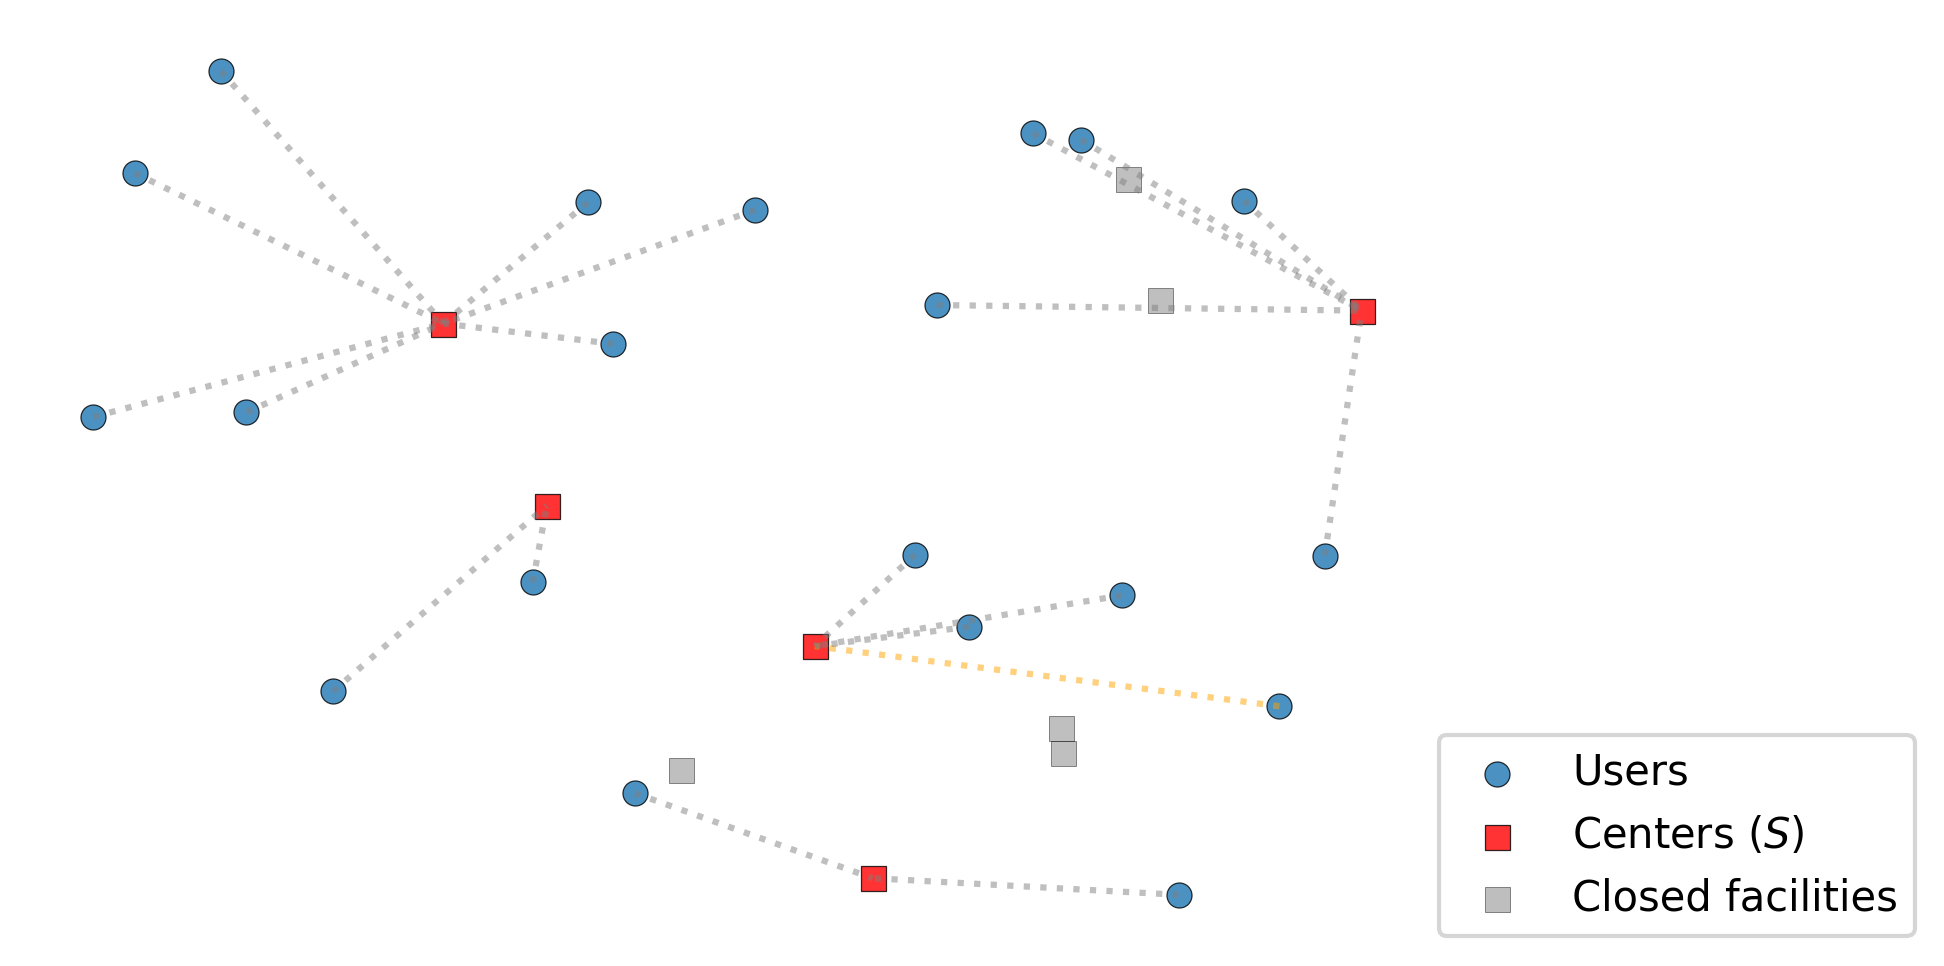
\includegraphics[scale=0.7]{1npcp}
        \label{fig:1npcp}
    \end{figure}
\end{frame}

\begin{frame}{Combinatorial model}
    \framesubtitle{Problem formulation}
    \begin{itemize}
        \item Sets and parameters
        \begin{itemize}
            \item $V = \{1, 2, ..., n\}$, set of nodes
            \item $d_{ij} = $ distance between nodes $i$ and $j$, $i,j \in V$
            \item $\alpha = $ position of closest assigned center for all $v \in V \setminus P$
        \end{itemize}
        
        \item Variables sets
        \begin{itemize}
            \item $P = \{c_1, c_2, ..., c_p\}$, set of centers
        \end{itemize}
    \end{itemize}
\end{frame}

\begin{frame}{Combinatorial model}
    \framesubtitle{Problem formulation}
    \begin{block}{Objective}
        $$
        \min\limits_{P \in \Pi} \,
        \max\limits_{v \in V \setminus P} \,
        \min\limits_{S \subseteq P, |S| = \alpha} \,
        \max\limits_{s \in S}{d(s, v)}
        $$
        
        $$2 \leq \alpha \leq p \leq |V|$$
    \end{block}
    
    where $\Pi$ is the collection of subsets of $V$ of cardinality $p$, that is, $\Pi = \{ P \subseteq V : |P|=p \}$.
\end{frame}

\begin{frame}{Applications}
    \begin{figure}
        \centering
        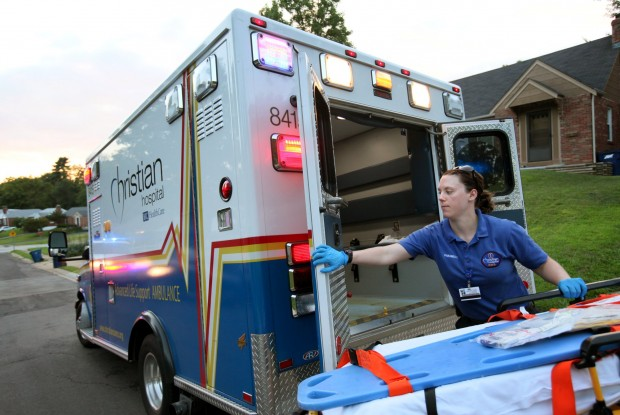
\includegraphics[scale=0.19]{ambulance}
        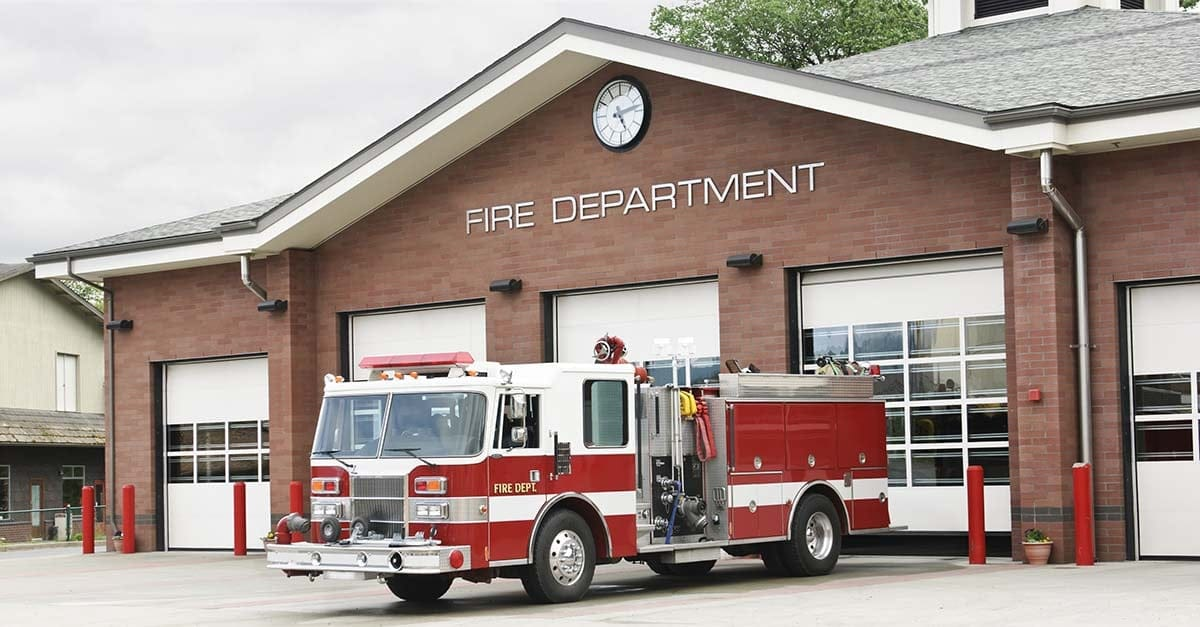
\includegraphics[scale=0.14]{fire_station}
    \end{figure}
    The aim is to have a minimum guaranteed response time between a customer or demand point and its $\alpha$-th closest center by considering a notion of fault tolerance, i.e., providing backup centers in case one of them fails to respond to an emergency situation.
    
    This ensures that even if up to $\alpha - 1$ facilities fail, every customer has a functioning facility close to it.
\end{frame}

\begin{frame}{Literature overview}
    The \anpcp has received less attention in the literature compared to the \pcp. There are optimal, approximation, and relaxation algorithms.
    To the best of our knowledge, there's only one heuristic approach for the general uncapacitated \anpcp and it's used to get lower and upper bounds for an optimal algorithm.
\end{frame}

\section{Proposed heuristic}

\begin{frame}{Proposed heuristic}
    \begin{columns}
        \column{0.6\textwidth}
        \begin{algorithmic}[1]
        
        \REQUIRE $V, d(i, j), p, \alpha, \beta, i_{max}$
        \ENSURE $P^*$ := set of $p$ centers
        
        \STATE $P^* \gets \emptyset$
        \STATE $f^* \gets \infty$
        \WHILE {$i_{max} > 0$}
            \STATE $P \gets$ Construct($V, d(i,j), \alpha, \beta$)
            \STATE $P \gets$ LocalSearch($P$)
            \IF {$f(P) < f^*$}
                \STATE $f^* \gets f(P)$
                \STATE $P^* \gets P$ 
            \ENDIF
            \STATE $i_{max} \gets i_{max} - 1$
        \ENDWHILE
        \RETURN $P^*$
        
        \end{algorithmic}
        
        \column{0.4\textwidth}
        A metaheuristic framework with a Greedy Randomized Adaptive Search Procedure (GRASP) using a value-based restricted candidate list (RCL).
        
        Parameters:
        \begin{itemize}
            \item $\beta$: Threshold quality parameter
            \item $i_{max}$: Number of iterations
        \end{itemize}
    \end{columns}
\end{frame}

\begin{frame}{Construction phase}
     Two constructive heuristics were implemented and compared to determine which of them will be used in further experimentation, i.e. as a previous step for a local search improvement or as an initial component of a metaheuristic framework.
\end{frame}

\begin{frame}{Construction phase}
    \framesubtitle{Greedy Dispersion (GD)}
    The first heuristic, called GD, is based on the $p$-dispersion problem (\pdp), which consists in selecting $p$ facilities from a given set of $n$ candidates in such a way that the minimum distance between facilities is maximized. It is of interest here because of how the facilities scatter among clients.
    
    \begin{block}{\pdp objective function}
        $$
        \max\limits_{P \subseteq V} \min\limits_{i,j \in P} d(i, j)
        $$
        
        $$p \leq |V|$$
    \end{block}
    
    The first two facilities are $i^*,j^* \gets \argmax\limits_{i,j \in V} d(i,j)$.
    
    Then, iteratively choose a node seeking the farthest node to the current solution, $v^* \gets \argmax\limits_{v \in V \setminus P} \min\limits_{s \in P} d(v, s)$
\end{frame}

\begin{frame}{Construction phase}
    \framesubtitle{Greedy Center (GC)}
    
    The second heuristic, called GC, evaluates the actual objective function of the \anpcp when choosing the next node to add to the solution.
    
    \begin{block}{\anpcp objective function}
        $$
        \min\limits_{P \in \Pi} \,
        \max\limits_{v \in V \setminus P} \,
        \min\limits_{S \subseteq P, |S| = \alpha} \,
        \max\limits_{s \in S}{d(s, v)}
        $$
        
        $$2 \leq \alpha \leq p \leq |V|$$
    \end{block}
\end{frame}

\begin{frame}{Local search}
    \begin{block}{move($s, v$)}
        \centering
        Interchange an assigned facility, $s \in P$, by an unassigned facility, $v \in V \setminus P$
    \end{block}
    
    Two strategies were coded and tested:
    \begin{itemize}
        \item Heuristic IF: move to the \textbf{first} improving neighbor.
        \item Heuristic IM: move to the \textbf{best} improving neighbor.
    \end{itemize}
\end{frame}

\section{Empirical work}

\begin{frame}{Experiments layout}
    \framesubtitle{Computational results}
    The heuristic was coded in Python 3.8.
    The source code can be found in the following repository: \url{https://github.com/netotz/alpha-neighbor-p-center-problem/}.
    The platform is Intel Core i5 2.3 GHz, 8 GB RAM under Windows 10, using CPython.
    For the experiments, instances were generated with nodes with random coordinates between 0 and 1000 for both axes.
\end{frame}

\begin{frame}{Constructive algorithms comparison}
    \framesubtitle{Computational results}

    \begin{block}{Data set}
        \begin{description}
            \item[Size 1] 20 instances with 50 total nodes and 5 to be located.
            \item[Size 2] 20 instances with 400 total nodes and 20 to be located.
        \end{description}
    \end{block}

    \begin{table}
        \centering
        \begin{tabular}{c|c|c|c|c|c|c}
            \hline
            \multicolumn{3}{c}{Instances} &
            \multicolumn{2}{|c|}{Avg. $f(P)$} &
            \multicolumn{2}{c}{Avg. time (s)} \\ \hline
            $n$ & $p$ & $\alpha$ & GD & GC & GD & GC \\ \hline
            \multirow{2}{*}{50} & \multirow{2}*{5} & 2 & 700.4 & 589.3 & 0 & 0.03 \\
            & & 3 & 843.0 & 714.6 & 0 & 0.01 \\ \hline
            \multirow{2}*{400} & \multirow{2}*{20} & 2 & 310.1 & 330.1 & 0.06 & 48.35 \\
            & & 3 & 381.0 & 410.5 & 0.06 & 38.98 \\
            \hline
        \end{tabular}
        \caption{Summary of the experiment results}
        \label{tab:constructive_exp}
    \end{table}
    
    Based on these results, it was decided to use the \pdp heuristic, GD, as the construction step for the GRASP framework.
\end{frame}

\begin{frame}{Local search performance}
    \framesubtitle{Computational results}
    
    The performance of both strategies of the local search heuristic was tested by trying to improve the solutions found by the constructive heuristic GD.

    \begin{table}
        \centering
        \scalebox{0.8}{
            \begin{tabular}{c|c|c|c|c|c|c|c|c|c|c}
                \hline
                \multicolumn{3}{c}{Instances} &
                \multicolumn{3}{|c}{Average $f(P)$} &
                \multicolumn{3}{|c}{Average time (s)} &
                \multicolumn{2}{|c}{Avg. rel. imp. (\%)} \\ \hline
                
                $n$ & $p$ & $\alpha$ & GD & IF & IM & GD & IF & IM & IF & IM \\ \hline
                
                \multirow{4}{*}{100} & \multirow{2}*{5} & 2 &
             	661.9 & 545.2 & 549.6 &
             	0 & 0.56 & 0.56 &
             	16.9 & 16.2 \\
                
                & & 3 &
                844.8 & 713.6 & 707.7 &
                0 & 0.47 & 0.56 &
                15.3 & 16.0 \\ \cline{2-11}

                & \multirow{2}*{10} & 2 &
                421.1 & 346.5 & 346.4 &
                0 & 0.66 & 0.65 &
                17.3 & 17.3 \\

                & & 3 &
                543.3 & 465.1 & 467.5 &
                0 & 0.69 & 0.74 &
                14.2 & 13.7 \\  \hline

                \multirow{4}{*}{500} & \multirow{2}*{25} & 2 &
                246.7 & 227.9 & 226.9 &
                0.1 & 123.5 & 121.0 &
                7.5 & 7.8 \\

                & & 3 &
                309.4 & 280.8 & 279.4 &
                0.1 & 147.9 & 151.9 &
                9.2 & 9.6 \\ \cline{2-11}

                & \multirow{2}*{50} & 2 &
                185.4 & 161.0 & 159.0 &
                0.4 & 64.7 & 66.2 &
                12.9 & 14.0 \\

                & & 3 &
                215.8 & 192.7 & 192.2 &
                0.3 & 97.1 & 109.8 &
                10.5 & 10.7 \\ \hline
            \end{tabular}
        }
        \caption{Summary of the experiment results}
        \label{tab:localsearch_exp}
    \end{table}
    
    Both local search strategies clearly improve the solution given by GD.
    Nevertheless, while time increases significantly, the improvement ratio does not.
\end{frame}

\begin{frame}{Calibrating GRASP iterations}
    \framesubtitle{Computational results}
    
    In order to gain insight about when the solutions yielded by the GRASP algorithm stop improving, we run an experiment with $i_{max} = 2000$ and $\beta = 0.4$ for 4 instances of size 100.
    
    \begin{figure}
        \centering
        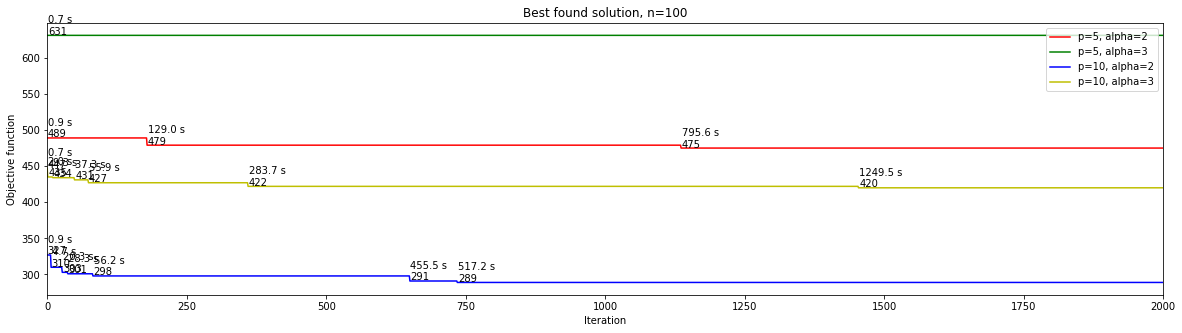
\includegraphics[scale=0.29]{grasp_iters_n100}
    \end{figure}
    
    As expected, most of the improvements and the most significant ones occur in the first iterations of GRASP.
    In general, after 250 iterations the objective function barely improved.
\end{frame}

\begin{frame}{Calibrating GRASP iterations}
    \framesubtitle{Computational results}
    
    For the same purpose as the previous one, another experiment was run, this time for one instance of size 300 with $i_{max} = 1000$ and $\beta = 0.4$.
    
    \begin{figure}
        \centering
        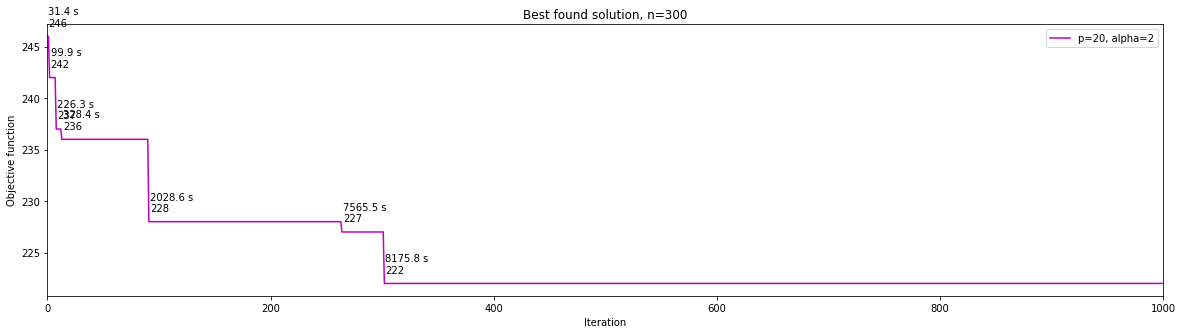
\includegraphics[scale=0.29]{grasp_iters_n300}
    \end{figure}
    
    Again, the relevant improvements took place in the first iterations.
    After 200 iterations there were no significant improvements.
    However, the time taken to reach the last improvement is extremely long.
\end{frame}

\section{Wrap-up}

\begin{frame}{Wrap-up}
    Conclusions
    \begin{itemize}
        \item Two constructive heuristics were proposed and tested
        \item Heuristics IF and IM showed better behaviour than heuristic GD
        \item A basic GRASP metaheuristic was presented
        \item On fine-tuning stage, it was observed that a value of $i_{max} = 250$ was good enough
        \item GRASP was applied to solve instances of up to $n = 100, p = 10$ in very reasonable running times
    \end{itemize}
    
    Future work
    \begin{itemize}
        \item Test heuristic against a lower bound to assess solution quality by using linear programming relaxation
        \item Improve the algorithm data structures to reduce running times
        \item Implement a reactive GRASP strategy
        \item Improve the metaheuristic by means of path relinking
    \end{itemize}
\end{frame}

\begin{frame}{Acknowledgments}
    \begin{itemize}
        \item Thank you very much for your attention!
        \item Feedback is welcome :)
        \item Email: neto.otz@hotmail.com
        \item GitHub: \url{https://github.com/netotz}
    \end{itemize}
    
    \begin{figure}
        \centering
        
\includegraphics[scale=0.2]{uanl-logo}
        
\includegraphics[scale=0.2]{fime-logo}
    \end{figure}
\end{frame}

\begin{frame}{References}
    \begin{thebibliography}{10}
        \bibitem{krumke1995} Krumke, S. O. (1995). On a generalization of the p-center problem. Information processing letters, 56(2), 67-71.
        \bibitem{medal2014} Medal, H. R., Rainwater, C. E., Pohl, E. A., \& Rossetti, M. D. (2014). A bi-objective analysis of the r-all-neighbor p-center problem. Computers \& Industrial Engineering, 72, 114-128.
        \bibitem{erkut1994} Erkut, E., Ülküsal, Y., \& Yenicerioğlu, O. (1994). A comparison of p-dispersion heuristics. Computers \& operations research, 21(10), 1103-1113.
        \bibitem{chen2013} Chen, D., \& Chen, R. (2013). Optimal algorithms for the $\alpha$-neighbor p-center problem. European Journal of Operational Research, 225(1), 36-43.
    \end{thebibliography}
\end{frame}

\end{document}
